\documentclass[xetex,mathserif,serif]{beamer}
\usepackage{polyglossia}
\setdefaultlanguage[babelshorthands=true]{russian}
\usepackage{minted}
\usepackage{tabu}

\useoutertheme{infolines}

\usepackage{fontspec}
\setmainfont{FreeSans}
\newfontfamily{\russianfonttt}{FreeSans}

\tabulinesep=0.7mm

\title{Порождающие и поведенческие паттерны, детали реализации}
\author[Юрий Литвинов]{Юрий Литвинов \newline \textcolor{gray}{\small\texttt{yurii.litvinov@gmail.com}}}

\date{26.04.2017г}

\begin{document}
	
	\frame{\titlepage}

	\section{Порождающие шаблоны}

	\begin{frame}
		\frametitle{``Фабричный метод'' (Factory Method), детали реализации}
		\begin{center}
			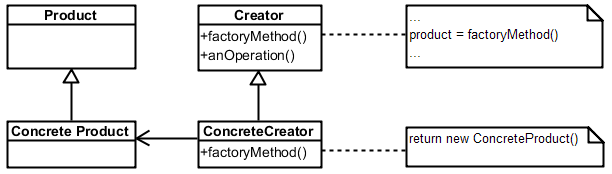
\includegraphics[width=0.6\textwidth]{factoryMethod.png}
		\end{center}
		\begin{itemize}
			\item Абстрактный Creator или реализация по умолчанию
			\begin{itemize}
				\item Второй вариант может быть полезен для расширяемости
			\end{itemize}
			\item Параметризованные фабричные методы
			\item Если язык поддерживает инстанциацию по прототипу (JavaScript, Smalltalk), можно хранить порождаемый объект
			\item Creator не может вызывать фабричный метод в конструкторе
			\item Можно сделать шаблонный Creator
		\end{itemize}
	\end{frame}

	\begin{frame}
		\frametitle{``Абстрактная фабрика'' (Abstract Factory), детали реализации}
		\begin{columns}
			\begin{column}{0.5\textwidth}
				\begin{itemize}
					\item Хорошо комбинируются с паттерном ``Одиночка''
					\item Если семейств продуктов много, то фабрика может инициализироваться \textit{прототипами}, тогда не надо создавать сотню подклассов
				\end{itemize}
			\end{column}
			\begin{column}{0.5\textwidth}
				\begin{center}
					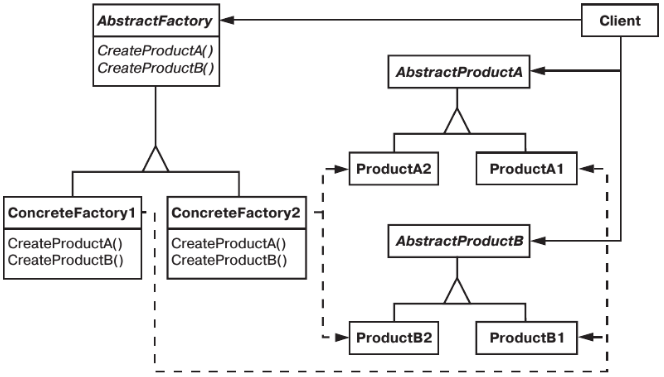
\includegraphics[width=\textwidth]{abstractFactory.png}
				\end{center}
			\end{column}
		\end{columns}
		\begin{itemize}
			\item Прототип на самом деле может быть классом (например, Class в Java)
			\item Если виды объектов часто меняются, может помочь параметризация метода создания
			\begin{itemize}
				\item Может пострадать типобезопасность
			\end{itemize}
		\end{itemize}
	\end{frame}

	\begin{frame}
		\frametitle{``Прототип'' (Prototype), детали реализации}
		\begin{itemize}
			\item Паттерн интересен только для языков, где мало runtime-информации о типе (C++)
			\item Реестр прототипов, обычно ассоциативное хранилище
			\item Операция Clone
			\begin{itemize}
				\item Глубокое и мелкое копирование
				\item В случае, если могут быть круговые ссылки
				\item Сериализовать/десериализовать объект (но помнить про идентичность)
			\end{itemize}
			\item Инициализация клона
			\begin{itemize}
				\item Передавать параметры в Clone --- плохая идея
			\end{itemize}
		\end{itemize}
	\end{frame}

	\begin{frame}
		\frametitle{``Строитель'' (Builder), детали реализации}
	\end{frame}

	\section{Поведенческие шаблоны}

	\begin{frame}
		\frametitle{``Шаблонный метод'' (Template Method), детали реализации}
		\begin{center}
			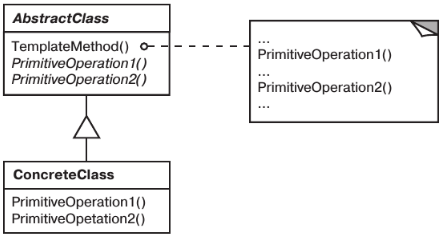
\includegraphics[width=0.5\textwidth]{templateMethod.png}
		\end{center}
		\begin{itemize}
			\item Сам шаблонный метод, как правило, невиртуальный
			\item Примитивные операции могут быть виртуальными или чисто виртуальными
			\begin{itemize}
				\item Лучше их делать protected
				\item Чем их меньше, тем лучше
			\end{itemize}
			\item Лучше использовать соглашения об именовании, например, называть операции с Do
		\end{itemize}
	\end{frame}

	\begin{frame}
		\frametitle{``Посредник'' (Mediator), детали реализации}
	\end{frame}

	\begin{frame}
		\frametitle{``Команда'' (Command), детали реализации}
	\end{frame}

	\begin{frame}
		\frametitle{``Цепочка ответственности'' (Chain of Responsibility), детали реализации}
	\end{frame}

	\begin{frame}
		\frametitle{``Наблюдатель'' (Observer), детали реализации}
	\end{frame}

	\begin{frame}
		\frametitle{``Состояние'' (State), детали реализации}
	\end{frame}

	\begin{frame}
		\frametitle{``Посетитель'' (Visitor), детали реализации}
	\end{frame}

	\begin{frame}
		\frametitle{``Хранитель'' (Memento), детали реализации}
	\end{frame}

	\begin{frame}
		\frametitle{``Интерпретатор'' (Interpreter), детали реализации}
	\end{frame}

	\begin{frame}
		\frametitle{``Итератор'' (Iterator), детали реализации}
	\end{frame}

	% \section{Антипаттерны}

	% \begin{frame}
	% 	\frametitle{Антипаттерны --- что это и зачем?}
	% 	\begin{itemize}
	% 		\item Часто встречающиеся решения, приводящие к известным проблемам
	% 		\begin{itemize}
	% 			\item Сами по себе решения могут быть неплохи, может быть плох контекст их применения
	% 		\end{itemize}
	% 		\item Так же, как и паттерны, нужны для введения общего словаря и общеизвестного набора решений
	% 		\item Описание антипаттерна должно содержать не только проблему, но и то, почему это решение плохо, и как сделать хорошо
	% 		\item Бывают разные виды, относящиеся к разным сферам деятельности
	% 		\begin{itemize}
	% 			\item Антипаттерны реализации
	% 			\begin{itemize}
	% 				\item В том числе, специфичные для конкретного языка или технологии
	% 			\end{itemize}
	% 			\item Архитектурные антипаттерны
	% 			\item Антипаттерны организации
	% 		\end{itemize}
	% 	\end{itemize}
	% \end{frame}

\end{document}